\documentclass[11pt,letterpaper]{article}
\PassOptionsToPackage{hyphens}{url}
\usepackage[margin=.83in,top=.8in,bottom=.8in,headheight=15pt]{geometry}
\usepackage[T1]{fontenc}
\usepackage{lmodern,amsmath,amssymb,mathtools,bm,booktabs,array,graphicx,tikz}
\usetikzlibrary{arrows.meta,positioning,calc,decorations.pathreplacing,patterns}
\definecolor{ink}{HTML}{17344D}\definecolor{accent}{HTML}{087E8B}\definecolor{pale}{HTML}{EDF5F5}\definecolor{gold}{HTML}{AD6B19}
\providecommand{\dd}{\,\mathrm{d}}\providecommand{\R}{\mathbb{R}}
\providecommand{\E}{\mathbb{E}}\providecommand{\Var}{\operatorname{Var}}
\providecommand{\Cov}{\operatorname{Cov}}\providecommand{\diag}{\operatorname{diag}}
\providecommand{\norm}[1]{\left\lVert#1\right\rVert}
\providecommand{\abs}[1]{\left|#1\right|}
\usepackage{microtype,hyperref,fancyhdr,enumitem,amsthm,sectsty,needspace}
\allsectionsfont{\raggedright}
\hypersetup{colorlinks=true,linkcolor=ink,urlcolor=accent,pdfauthor={Zan Ahmad},pdftitle={Muscle force and the pressure--volume cycle / Lecture notes}}
\setlength{\parindent}{0pt}\setlength{\parskip}{6pt}\linespread{1.07}
\setlist{itemsep=3pt,topsep=4pt,leftmargin=*}
\emergencystretch=2em\clubpenalty=10000\widowpenalty=10000
\pagestyle{fancy}\fancyhf{}\fancyhead[L]{\small Mathematical Cardiology}\fancyhead[R]{\small Lecture 3}
\fancyfoot[L]{\footnotesize Zan Ahmad}\fancyfoot[R]{\footnotesize\thepage}\renewcommand{\headrulewidth}{.3pt}
\newtheorem{proposition}{Proposition}\newtheorem{theorem}{Theorem}\newtheorem{lemma}{Lemma}
\theoremstyle{definition}\newtheorem{definition}{Definition}\newtheorem{example}{Example}
\numberwithin{equation}{section}
\begin{document}
{\small\scshape Mathematical Cardiology\hfill Lecture 3}\par\medskip
{\raggedright\hyphenpenalty=10000\exhyphenpenalty=10000\LARGE\bfseries\color{ink} Muscle force and the pressure--volume cycle\par}\medskip
{\small Lecture notes}\par\bigskip
The heart transfers mechanical energy to blood. To understand that statement, we must connect two scales without confusing them: force generated by muscle and pressure--volume work performed by a chamber. A muscle force--velocity curve and a ventricular pressure--volume loop are different experiments. We shall calculate what each measures and identify the additional assumptions that would be needed to connect them.

\section{From crossbridges to a macroscopic force}
\hypertarget{note-from-crossbridges-to-a-macroscopic-force}{}\label{note:from-crossbridges-to-a-macroscopic-force}
{\small \href{slides.html\#frame=two-levels-of-a-pumping-system\&step=1}{Slides for this section}}\par
Actin and myosin filaments slide relative to one another; the filaments do not have to shorten to make the muscle shorten. Myosin heads attach, develop force and detach. Many such interactions contribute to the force of a cell, while chemical energy supports their cycling. Activation and calcium regulation influence the available interactions. A ventricular wall adds geometry, fiber orientation and time-dependent activation to this microscopic description.

A useful accounting model groups attached crossbridges by their extension. Suppose $N$ is the number of available crossbridges, fraction $a_j$ are attached in extension group $j$, and one crossbridge in that group contributes force $f_j$. Then
\begin{equation}
F=N\sum_j a_j f_j,\qquad a_j\ge0,\quad\sum_j a_j\le1.
\end{equation}
The remaining fraction is unattached. This weighted sum explains why force depends on both the number attached and their mechanical state. It does not yet supply the attachment rates or the change of extension during sliding. The textbook develops those additional dynamics for a skeletal-muscle idealization. Here the sum provides a bridge between microscopic events and a macroscopic quantity without pretending to be a complete cardiac model.
\section{Normalize the force--velocity relation}
\hypertarget{note-normalize-the-force-velocity-relation}{}\label{note:normalize-the-force-velocity-relation}
{\small \href{slides.html\#frame=a-load-speed-family\&step=1}{Slides for this section}}\par
At approximately fixed activation, a muscle shortens more slowly against a larger resisting load over its shortening range. The isometric endpoint has nonzero force but zero shortening speed; zero speed is not zero force. A common family of illustrative relations has the form
\[
v=b\frac{F_0-F}{F+a},\qquad a,b>0,
\]
where $F_0$ is the isometric force. At zero load, $v_{\max}=bF_0/a$. Define $f=F/F_0$, $u=v/v_{\max}$ and $\alpha=a/F_0$. Dividing the relation by the unloaded speed gives
\begin{equation}
u=\frac{\alpha(1-f)}{f+\alpha}.
\end{equation}
Choosing $\alpha=1/3$ produces the plotted teaching curve $u=(1-f)/(1+3f)$, for $0\le f\le1$. It returns $u=1$ at zero load, $u=0$ at isometric load, and $u=0.2$ at $f=1/2$.

External shortening power is force times speed, so its normalized value is $fu$. It is zero at both endpoints: there is no load at one and no shortening at the other. At $f=1/2$, it is $0.1$ in these normalized units. This does not imply that biochemical energy consumption vanishes at either endpoint. The curve is not fitted to a patient and is not coupled to the chamber loop below.
\begin{center}\begin{minipage}{.98\linewidth}\centering
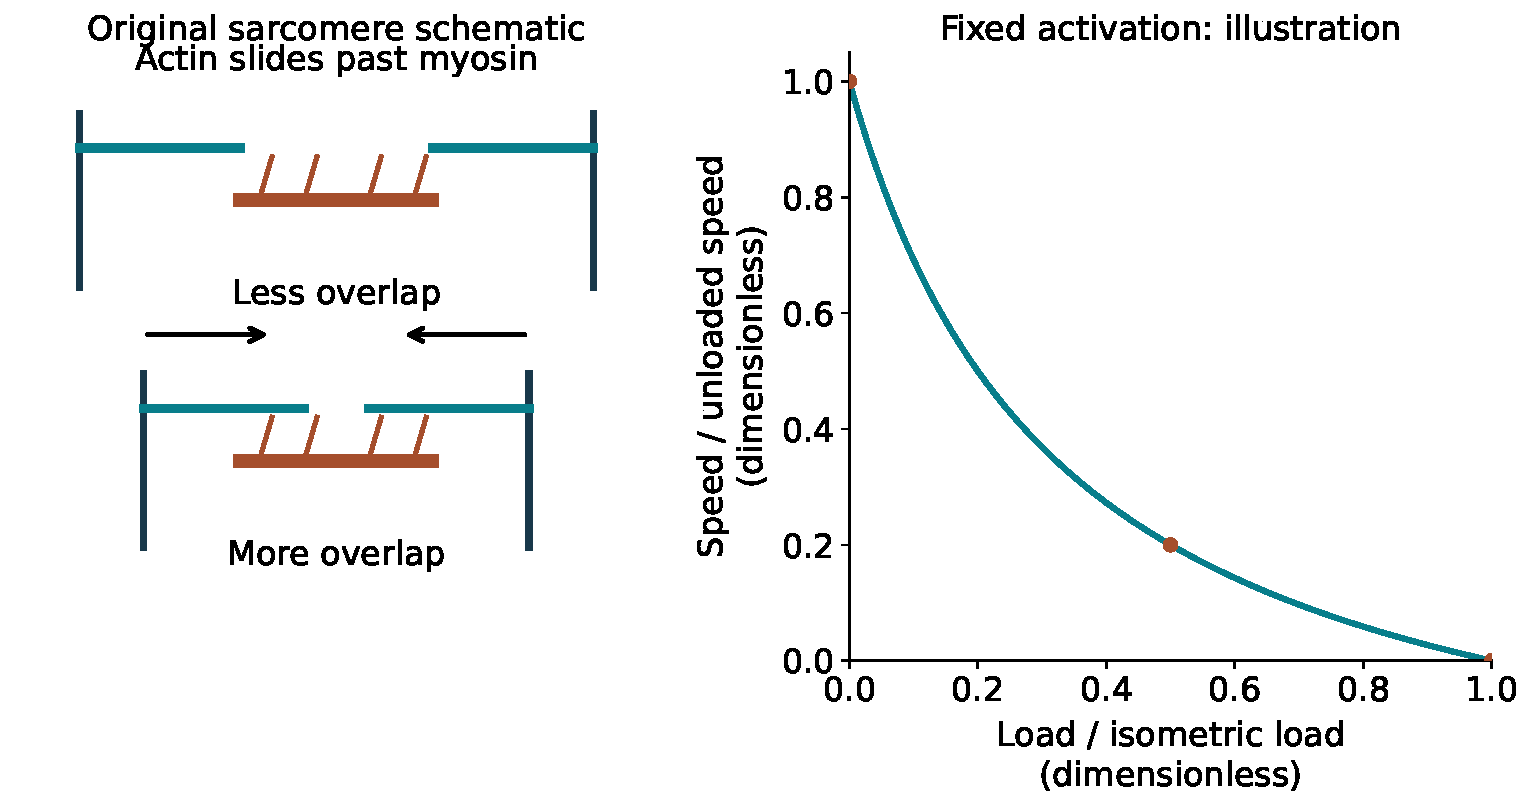
\includegraphics[width=.96\linewidth,height=.57\textheight,keepaspectratio]{muscle-and-load.pdf}\par\smallskip
{\small Original sliding-filament schematic and illustrative normalized curve u =\allowbreak{} (1 - f)/(1 +\allowbreak{} 3f). The curve is not calibrated cardiac mechanics and is not coupled to the loop.}
\end{minipage}\end{center}
\section{A loop records two state variables}
\hypertarget{note-a-loop-records-two-state-variables}{}\label{note:a-loop-records-two-state-variables}
{\small \href{slides.html\#frame=the-pv-plane-figure\&step=1}{Slides for this section}}\par
Put chamber volume on the horizontal axis and pressure on the vertical axis. A point $(V,P)$ represents one chamber state; a directed path records successive states. Horizontal distance is a volume change, not elapsed time. Two segments of equal length on the page need not take equal durations.

For the ideal left-ventricular cycle, filling occurs with the mitral valve open and the aortic valve closed. Volume rises at low pressure. Next, both valves are closed while pressure rises at nearly fixed chamber volume: isovolumic contraction. Ejection follows with the aortic valve open and the mitral valve closed; chamber volume falls. Finally, both valves close while pressure falls at nearly fixed volume. In this ideal picture the valves enforce direction in response to pressure differences.

The supplied rectangle prescribes a low pressure of $10$ mmHg, a high pressure of $100$ mmHg, and volumes from $50$ to $120$ mL. It omits rounded transitions, varying pressure during filling and ejection, regurgitation and detailed wall mechanics. Isovolumic refers to total chamber volume; it does not assert that every microscopic component is motionless.
\begin{center}\begin{minipage}{.98\linewidth}\centering
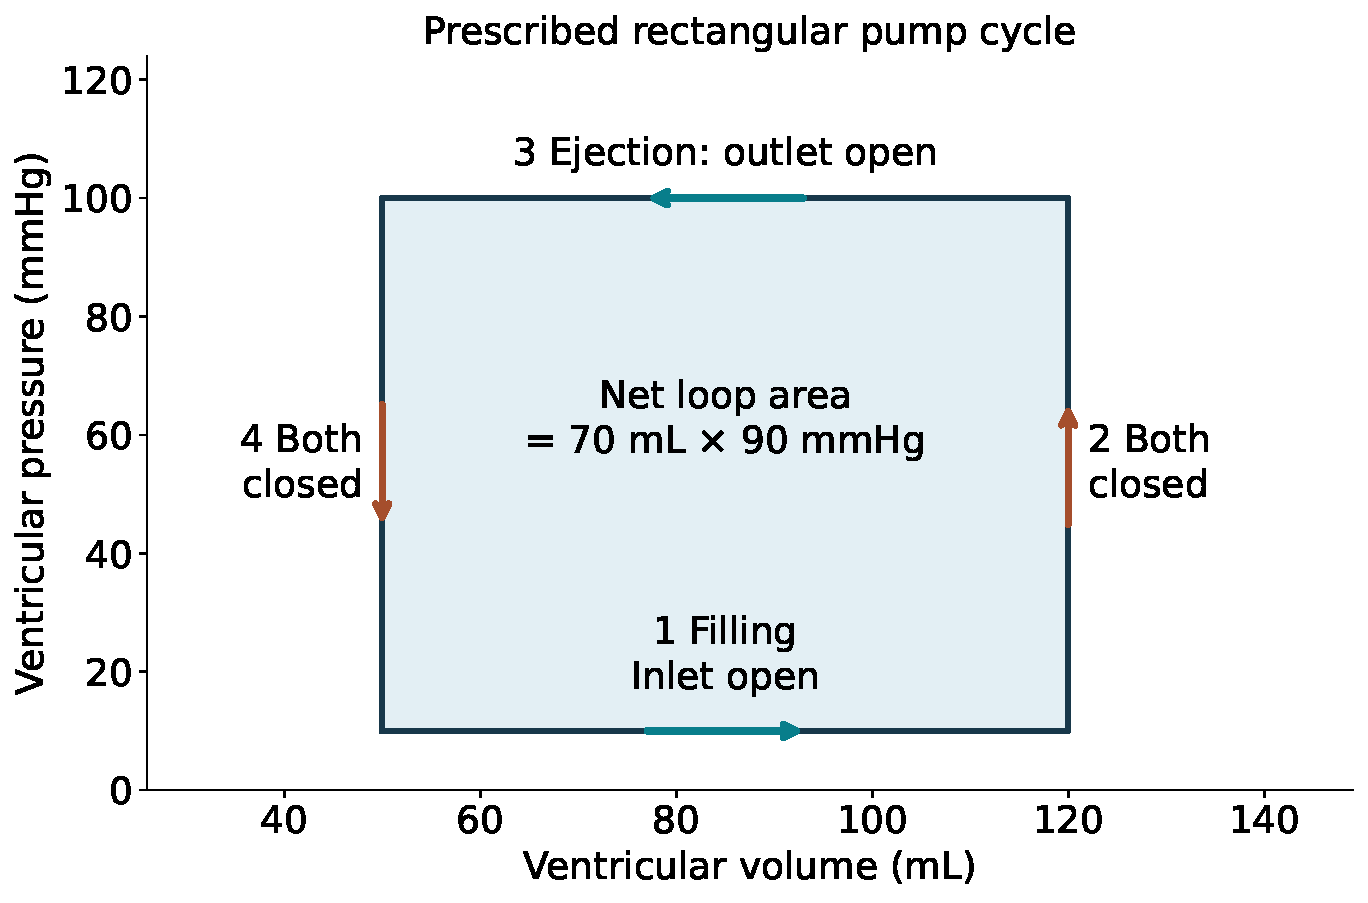
\includegraphics[width=.96\linewidth,height=.57\textheight,keepaspectratio]{pump-cycle.pdf}\par\smallskip
{\small Prescribed volumes 50--120 mL and pressures 10--100 mmHg. Arrows trace filling, closed-valve pressure rise, ejection and closed-valve relaxation.}
\end{minipage}\end{center}
\section{Stroke volume, ejection fraction, and output}
\hypertarget{note-stroke-volume-ejection-fraction-and-output}{}\label{note:stroke-volume-ejection-fraction-and-output}
{\small \href{slides.html\#frame=the-ejected-volume\&step=1}{Slides for this section}}\par
Let $EDV$ be the volume before ejection and $ESV$ the volume after it. With no regurgitant flow, the stroke volume is
\[
SV=EDV-ESV=120-50=70\ \mathrm{mL/beat}.
\]
The ejection fraction is a fraction of the starting chamber volume:
\[
EF=\frac{EDV-ESV}{EDV}=1-\frac{ESV}{EDV}
=\frac{70}{120}\approx0.583.
\]
It is dimensionless. It is not an energy-conversion efficiency. Two chambers can have the same fraction and different stroke volumes: scaling both $EDV$ and $ESV$ by the same positive factor preserves $EF$ while scaling $SV$.

If the prescribed beat repeats $75$ times per minute, average output is $70(75)=5250$ mL/min, or $5.25$ L/min. This multiplication assumes the same per-beat stroke volume. A physiological rate change can alter filling and ejection, so the arithmetic is not itself a law fixing stroke volume at higher rates.
\Needspace{10\baselineskip}

\section{Derive work from displaced volume}
\hypertarget{note-derive-work-from-displaced-volume}{}\label{note:derive-work-from-displaced-volume}
{\small \href{slides.html\#frame=why-pressure-times-volume-is-work\&step=1}{Slides for this section}}\par
For fluid displaced against pressure $P$, force times distance can be rewritten as pressure times volume: $(P A)\Delta x=P\Delta V$, where $A$ is the moving cross-sectional area. During ejection the chamber volume decreases, so positive work delivered by the chamber has contribution $-P\Delta V$ under the chamber-volume sign convention.

For the rectangle, ejection delivers $100(70)=7000$ mmHg mL. Filling at $10$ mmHg contributes $-10(70)=-700$ mmHg mL to work delivered by the chamber. The vertical segments have $\Delta V=0$. Consequently
\begin{equation}
W_{\rm net}=(100-10)(120-50)=6300\ \mathrm{mmHg\,mL}.
\end{equation}
Using $1\ \mathrm{mmHg\,mL}\approx1.33322\times10^{-4}$ J gives approximately $0.840$ J per cycle. This is the area enclosed by the prescribed rectangle.

For a curved loop, partition the path into small volume changes and add $-P_j\Delta V_j$. In calculus notation the limiting sum is $-\oint P\,dV$ with the stated orientation. The area interpretation can therefore be understood without assuming a rectangular physiological loop. Axis units and scales matter; the physical work is not the raw area measured in square centimeters on the printed page.
\section{Coupling muscle mechanics to chamber work}
\hypertarget{note-coupling-muscle-mechanics-to-chamber-work}{}\label{note:coupling-muscle-mechanics-to-chamber-work}
{\small \href{slides.html\#frame=coupling-force-geometry-and-pressure\&step=1}{Slides for this section}}\par
The crossbridge picture motivates active force, and the loop calculates chamber-level work. Neither is a derivation of the other in this lesson. Connecting them requires an activation model, tissue mechanics, chamber geometry and coupling to the surrounding circulation. Likewise, net pressure--volume work is only one contribution to the energetic demand of myocardium. Isovolumic contraction may require active force even though its chamber-volume work is zero.

A closed prescribed loop should eject the same volume that it receives over a cycle. Its rectangle area should agree with an independent polygon-area calculation. These check consistency of the constructed example. To compare with a real heart, pressure and volume measurements must share a time base and a calibrated volume scale. A project can compare alternative loop shapes and determine which geometric changes alter work while preserving stroke volume; that is a more specific claim than treating every larger loop as evidence of improved cardiac function.
\bigskip
\section*{Exercises}
\par\noindent\begin{minipage}{\linewidth}
\subsection*{MC03-E1. Interpret a new loop}
A prescribed cycle has EDV 130 mL, ESV 65 mL and heart rate 80 beats/min, with no valve leakage.

\textbf{a} Calculate stroke volume and ejection fraction.

\end{minipage}\par\medskip
\textbf{b} Calculate output in L/min.

\textbf{c} State the valve condition during a vertical pressure-rise segment and explain why its chamber volume stays fixed.

\par\noindent\begin{minipage}{\linewidth}
\subsection*{MC03-E2. Area and energy}
A rectangular loop spans 60--110 mL and 8--88 mmHg. Use 1 mmHg mL =\allowbreak{} 0.000133322 J.

\textbf{a} Compute net loop work in mmHg mL and joules.

\end{minipage}\par\medskip
\textbf{b} If the prescribed pressure height doubles while width stays fixed, what happens to work?

\textbf{c} Explain why zero volume-work during a vertical segment does not imply zero metabolic energy use, and why the doubled rectangle does not predict a real response to increased arterial load.

\par\noindent\begin{minipage}{\linewidth}
\subsection*{MC03-E3. Mechanism, model and project}
Use the original sliding-filament sketch and the illustrative fixed-activation load-speed curve.

\textbf{a} Describe what changes and what stays fixed when the drawn sarcomere shortens.

\end{minipage}\par\medskip
\textbf{b} For f =\allowbreak{} 1/3, compute u =\allowbreak{} (1 - f)/(1 +\allowbreak{} 3f). What does the isometric endpoint mean?

\textbf{c} Propose a testable loop-area project and identify one independent measurement and one limitation.

\section*{References}
\noindent\begin{minipage}{\linewidth}
Zan Ahmad, Fall 2023 HEART syllabus. Public PDF pp. 1--2, Course Topics and Course Expectations; editable syllabus pp. 2--3, project requirements.

\end{minipage}\par\medskip
\noindent\begin{minipage}{\linewidth}
Hoppensteadt and Peskin, Modeling and Simulation in Medicine and the Life Sciences, second edition. Printed pp. 171--174; PDF pp. 184--187, sections 5.1--5.2.

\end{minipage}\par\medskip
\noindent\begin{minipage}{\linewidth}
NHLBI, How the Heart Beats. The conduction system and heartbeat description.

\url{https://www.nhlbi.nih.gov/health/heart/heart-beats}
\end{minipage}\par\medskip
\end{document}
